\chapter{Grundlagen}\label{ch:related_work}
%alles was man braucht um den rest zu verstehen

\section{Statische Ressourcen}
Statische Ressourcen sind Inhalte einer Website die für alle Nutzer gleich sind. Sie sind im Gegensatz zu dynamischen Inhalten nicht nutzerspezifisch und können daher gut über ein CDN verteilt werden. Insbesondere die so genannten Assets einer Internetseite sind meist statisch. Dies sind meist Javascript, CSS aber auch Bild Dateien. Auch Videos fallen häufig in diese Kategorie.

\section{\cdn}
Unter einem \cdn, auch Content Delivery Network versteht man ein Netzwerk in dem sich Clients Inhalte von einer Reihe von Knoten laden. Ein \cdn stellt dem Nutzer Auslieferungs und Speicherkapazitäten zur Verfügung. Dadurch kann die Last auf dem Ursprungsserver und die Latenz auf Seiten der Nutzer reduziert werden. Die reduzierten Ladezeiten werden unter anderem durch eine bessere geographische Nähe und damit geringerer Netzlaufzeiten erreicht. %TODO: gute definition finden

Es lassen sich drei Klassen von \cdns unterscheiden. Infrastuktur basierte CDN die auf einer geografisch verteilten Server Infrastruktur basieren, \pTp basierte \cdns bei denen die Inhalte direkt zwischen den Teilnehmern verteilt werden und Hybride \cdns die aus einer Kombination aus Server Infrastruktur und \pTp Verteilung beruhen.

%- Content Distribution Network
%- Servernetzwerk das inhalte lokal verteilt
%- reduzierung der physischen Entfernung
%- bereitstellung von auslieferkapazitäten
\subsection{Infrastruktur basierte \cdns}
Infrastruktur basierte \cdns bestehen aus einem Ursprungsservern, der von dem Bereitsteller der Inhalte kontrolliert wird, und einem Netzwerk aus replica Servern. Die replica Server übernehmen die Verteilung der Inhalte an die Clients. Sie fungieren als ein möglichst regionaler cache in dem Inhalte des Ursprungsservers gespiegelt werden. Ein Distributionssystem ist dafür verantwortlich die Inhalte auf den replicas zu aktuallisieren und übernimmt das Routing bei einer Anfrage eines Clients. Unter Zuhilfenahme verschiedener Metriken versucht das Distributionssystem einen möglichst optimalen replica Server für den Client zu finden. Diese Metriken unterscheiden sich zwischen den Anbietern. Häufig werden jedoch geographische Entfernung, Latenzzeiten und die Übertragungsrate berücksichtigt. Um eine möglichst geringe Latenz zu erreichen sind infrastruktur basierte \cdns häufig geografisch sehr verteilt und bestehen aus meherern tausend replica Servern. So hat Akamai, einer der größten \cdn Anbietern, über 137000 Server in 87 Ländern. \cite{akamaiPeer} 

%-ein ursprungsserver
%- viele replicaserver
%- request routing system wählt optimalen replica server
%- ua. nach geographische Entfernung, Latenzzeit, Übertragungsrate
%137,000 servers in 87 countries
%within over 1,150 Internet networks, \cite{akamaiPeer}

%https://de.wikipedia.org/wiki/Content_Delivery_Network
\subsection{\pTp basierte \cdns }

Bei einem \pTp Netzwerk handelt es sich um eine Netzwerk Struktur bei der alle Teilnehmer gleichberechtigt sind. Sie bildet damit das gegen Konzept zur klassischen Client-Server Struktur, bei der einer oder mehrere Server einen Dienst anbieten der von Clients genutzt werden kann. In einem \pTp Netzwerk können die Teilnehmer sowohl Dienste anbieten als auch nutzen. Man unterscheidet zwischen unstrukturierten und strukturierten \pTp Netzwerken. 

Unstrukturierte Netzwerke haben keine Zuordnung von Objekten und Teilnehmern. Es ist nicht möglich gezielt nach einem Objekt zu suchen. Sie lassen sich einteilen in zentralisierte, reine und hybride \pTp Netzwerke. Zentralisierte Netze haben zur Verwaltung einen Server der unter anderem die Verbindung der Teilnehmer übernimmt. Dadurch ist es möglich eine Verbindung aufzubauen ohne das die IP Adresse im Vorfeld bekannt ist. Reine \pTp Netzwerke haben keinen zentralen Verwaltungsserver. Die Verwaltung des Netzwerkes wird von den Teilnehmern selber übernommen. Das hat zur Folge das eine Verbindung nur möglich ist, wenn die IP Adresse des anderen Teilnehmers bekannt ist. 

Strukturierte \pTp Netzwerke haben eine Zuordnung von Objekt und Teilnehmer. Es ist also möglich gezielt nach einem Objekt zu suchen. Dies wird häufig über verteilte Hash Tabellen, über die mit einem verteilten Index gesucht werden kann, realisiert.


Typische wenn auch nicht notwendige Charakteristika sind laut Steinmetz\cite{p2pBook2005}:

\begin{itemize}
  \item Heteorogenität der Internetbandbreite der Teilnehmer
  \item Verfügbarkeit und Qualität der Verbindung zwischen Teilnehmern kann nicht vorausgesetzt werden
  \item Dienste werden von den Teilnehmern angeboten und genutzt
  \item Die Teilnehmer bilden ein Netz das auf ein bestehendes Netz aufgesetzt wird(Overlay Netzwerk) und stellen Suchfunktionen bereit
  \item Es besteht eine Autonomie der Teilnehmer bei der Bereitstellung von Ressourcen
  \item Das System ist selbstorganisiert
  \item Die restlichen Systeme müssen nicht skaliert werden und bleiben intakt
\end{itemize}

Reine \pTp \cdn Systeme sind im Kontext von Internet Anwendungen eher selten zu finden. Ein klassischer Anwendungsfall für diese Systeme ist das Filesharing.


%
%
%test \cite{p2pBook2005}
% https://de.wikipedia.org/wiki/Peer-to-Peer#Typen_von_Peer-to-Peer-Systemen
%gegenmodell zu client server
%gleichbererchtigte teilnehmer eines rechnernetzwerkes
%overlays erklären??
%häufig aufgabenverteilung der peers
%unstrukturierte p2p:
%	keine peer objekt zuordnung
%	zentralisierte p2p netzwerke - server zur verwaltung
%	reine p2p netzwerke - keine verbindung zu unbekannten ips
%	hybride p2p n. mehere zentrale server die dynamisch zugeteilt werden
%	zenralisierte und reine p2p netzwerke 1.gen. 
%strukturierte p2p:
%	objektzuordnung vorhanden --> suche möglich
%	oft verteilte hashtabellen --> verteilter index

%Peers weisen eine hohe Heterogenität bezüglich der Bandbreite, Rechenkraft, Online-Zeit, … auf.
%Die Verfügbarkeit und Verbindungsqualität der Peers kann nicht vorausgesetzt werden („Churn“).
%Peers bieten Dienste und Ressourcen an und nehmen Dienste anderer Peers in Anspruch (Client-Server-Funktionalität).
%Dienste und Ressourcen können zwischen allen teilnehmenden Peers ausgetauscht werden.
%Peers bilden ein Overlay-Netzwerk und stellen damit zusätzliche Such-Funktionen zur Verfügung.
%Peers haben eine signifikante Autonomie (über die Ressourcenbereitstellung).
%Das P2P-System ist selbstorganisierend.
%Alle übrigen Systeme bleiben konstant intakt und nicht skaliert.
\subsection{Hyrid \cdns}
Hybrid \cdns kombinieren \pTp \cdns und Infrastuktur basierte \cdns. Bei hybriden \cdns wird zuerst versucht die Resource über das Peer Netzwerk zu laden. Ist dies nicht möglich wird auf ein Infrastruktur basiertes \cdn zurück gegriffen. Dadurch kann die Last auf dem \cdn verringert und durch die Kombination verschiedener \cdns eine bessere Ausfallsicherheit erreicht werden. Häufig kommt diese Art der \cdns zum Einsatz wenn Ressourcen für Websites mit einem \pTp Ansatz verteilt werden sollen. Da in diesem Kontext nicht alle Teilnehmer die technischen Vorraussetzungen mitbringen um an dem \pTp Netzwerk teilzunehmen ist eine entsprechende alternative Lösung nötig. Da die viele Websites bereits mit einem Infrastruktur basierten \cdn arbeiten ist es naheliegend dieses weiter zu verwenden.

\section{\webrtc - Web Real-Time Communication}

\webrtc ist ein Framework mit dem Echtzeit Kommunikation zwischen Browser und mobilen Anwendungen ermöglicht wird. Mit Hilfe von \webrtc ist es möglich eine \pTp Verbindung aufzubauen und Daten direkt zwischen den Clients auszutauschen ohne das externe Plugins erforderlich sind. Insbesondere der Austausch von Multimedia Inhalten soll ermöglicht werden. Neben der Unterstützung für video und audio Inhalten gibt es jedoch auch die Möglichkeit Daten auszutauschen. \webrtc ist ein vom W3C\cite{w3Webrtc} standarisierter offener Standart an dem seit Frühjahr 2011 gearbeitet wird. Aktuell wird \webrtc von Chrome, Firefox, Android und iOS unterstützt.\footnote{https://caniuse.com/\#feat=rtcpeerconnection} \webrtc implementiert drei APIs: MediaStream, RTCPeerConnection und RTCDataChannel die im folgenden genauer beschrieben werden.

% SSl erwähnen
% Server wird durch pTp gespart 
% TODO: SSL erklären???


%https://de.wikipedia.org/wiki/WebRTC
%https://www.w3.org/TR/webrtc/
%https://webrtc.org/


\subsection{RTCPeerConnection}

% RTCPeerConnection is used to connect peers across the internet.

\subsection{RTCDataChannel}

% Übertragung von allem was nicht audio oder video ist. zb. text von chats
% support für string, blob, arraybuffer, ArrayBufferView

% RTCDataChannel uses Stream Control Transmission Protocol (SCTP)
% RTCDataChannel can work in unreliable and unordered mode (analogous to User Datagram Protocol or UDP), reliable and ordered mode (analogous to Transmission Control Protocol or TCP) and partial reliable modes:
% Reliable and ordered mode guarantees the transmission of messages and also the order in which they are delivered. This takes extra overhead, thus potentially making this mode slower.
% Unreliable and unordered mode does not guarantee every message will get to the other side nor what order they get there. This removes the overhead, allowing this mode to work much faster.
% Partial reliable mode guarantees the transmission of message under a specific condition (such as a retransmit timeout or a maximum amount of retransmissions). The ordering of messages is also configurable.

% https://bloggeek.me/sctp-data-channel/
\subsection{MediaStream}
Die Mediastream api, auch getUserMedia, ermöglicht es Echtzeit Daten wie audio oder Video aufzunehmen, anzuzeigen und an andere Clients weiter zu leiten und repräsentiert Medien Streams wie z.b. Audio oder Video Streams. Sie ermöglicht unter anderem den Zugriff auf Video Kameras und Mikrofone. Durch Sie ist es möglich auf die Hardwareunterstützung für Videos mittels open GL zuzugreifen. MediaStreams lassen sich mithilfe des src Attributes von HTML 5 video Elementen in das DOM einbinden. MediaStreams wurden von vom W3C in einem eigenen Standart definiert.\cite{w3MediaStream} 

\subsection{Singaling}

%https://www.html5rocks.com/en/tutorials/webrtc/infrastructure/#what-is-signaling

% For signaling: to enable the exchange of media and network metadata to bootstrap a peer connection.

\subsection{SDP}

\subsection{TURN Server}
% TURN servers (if direct connection fails and data relaying is required).

\subsection{STUN Server - Simple Traversal of User Datagram Protocol [UDP] Through Network Address Translators}

Da die Anzahl von IPv4 Adressen begrenzt ist, verwenden die meisten Subnetze NATs. Das hat zur folge das diese Clients nicht wissen wie über welche IP Adresse und welchen Port sie erreichbar sind. Daher ist der Einsatz von STUN Servern nötig um einen Verbindungsaufbau zu ermöglichen. Stun Server überprüfen eingehende Anfragen auf IP Adresse und Port und senden diese Informationen zurück an den Client, der somit in der Lage ist diese Information weiter zureichen und damit auch außerhalb seines lokalen Netzwerkes erreichbar ist. Das STUN-Protokoll ist im RFC 3489 \cite{rfcStun} definiert und ist nicht auf Webrtc beschränkt.


% TODO: evtl NATs erklären
%not enough IPv4 addresses
%→ most clients behind NATs, not reachable directly by IP address
%
%client behind NATs can’t know how they can get accessed from the internet
%→ using STUN server
%
%STUN servers check the IP and port of incoming request and send the information back

\subsection{ICE}

%setting: 2 peers, signaling server, STUN server
%each peer has a variety of candidate transport addresses (IP:port) 
%addresses from directly attached network (host candidate)
%translated transport (server reflexive) address
%ICE determine  which pairs of addresses work and which connection should be used
%try all possible pairs in smart order

\section{DataCache}

% https://www.w3.org/TR/DataCache/

\section{IndexedDB}

IndexedDB ist ein HTML 5 Feature um Daten im Browser zu speichern. Es wurde vom W3C standarisiert\cite{w3IndexedDB} und soll den veralteten websql standard ablösen. Im gegensatz zu websql hat die IndexedDB keine strukturierte Query Language und ihr liegt kein relationelles Modell zu grunde. Sie stellt einen Key-Value Store bereit der in der Lage ist auch große Datenmengen effektiv bereit zu stellen. Dabei ist der Datenzugriff auf die selbe Domain beschränkt. Die API ist überwiegend asyncron und basiert auf Promises.

\section{Service Worker}
Service Worker sind Skripte die im Browser als separate Prozesse im Hintergrund laufen, so genannte Web Worker. Sie stellen die Funktionalitäten eines programmierbaren Netwerk Proxies bereit. Durch Service Worker ist es möglich die Anfragen einer Seite zu kontrollieren auf sie zu reagieren und in den Prozess einzugreifen.\cite{w3ServiceWorker} Service Worker haben keinen Zugriff auf das DOM. Sie könne mehrere Browser-Tabs und mit Hilfe des PostMessage Protokolls können Nachrichten zwischen Service Worker und Browser-Tab ausgetauscht werden. Da Service Worker Zugriff auf den DataCache und die IndexDB haben werden sie häufig verwendet um Internetseiten offline verfügbar zu machen. Bei der Registrierung eines Service Workers wird ein URL-Scope fest gelegt für den der Service Worker zuständig ist. Nur Anfragen die sich innerhalb des URL-Scopes des Service Workers befinden können von diesem bearbeitet werden.

%nur zugriff auf inhalte unterhalb der domain(nur gleiche domain)
%fetch event
%werden gestartet und gestoppt --> kein zuverlässiger globaler zustand
%having access to IndexDB
%https wird benötigt
\subsection{Lebenszyklus}
\begin{figure}[!h]
	\centering
	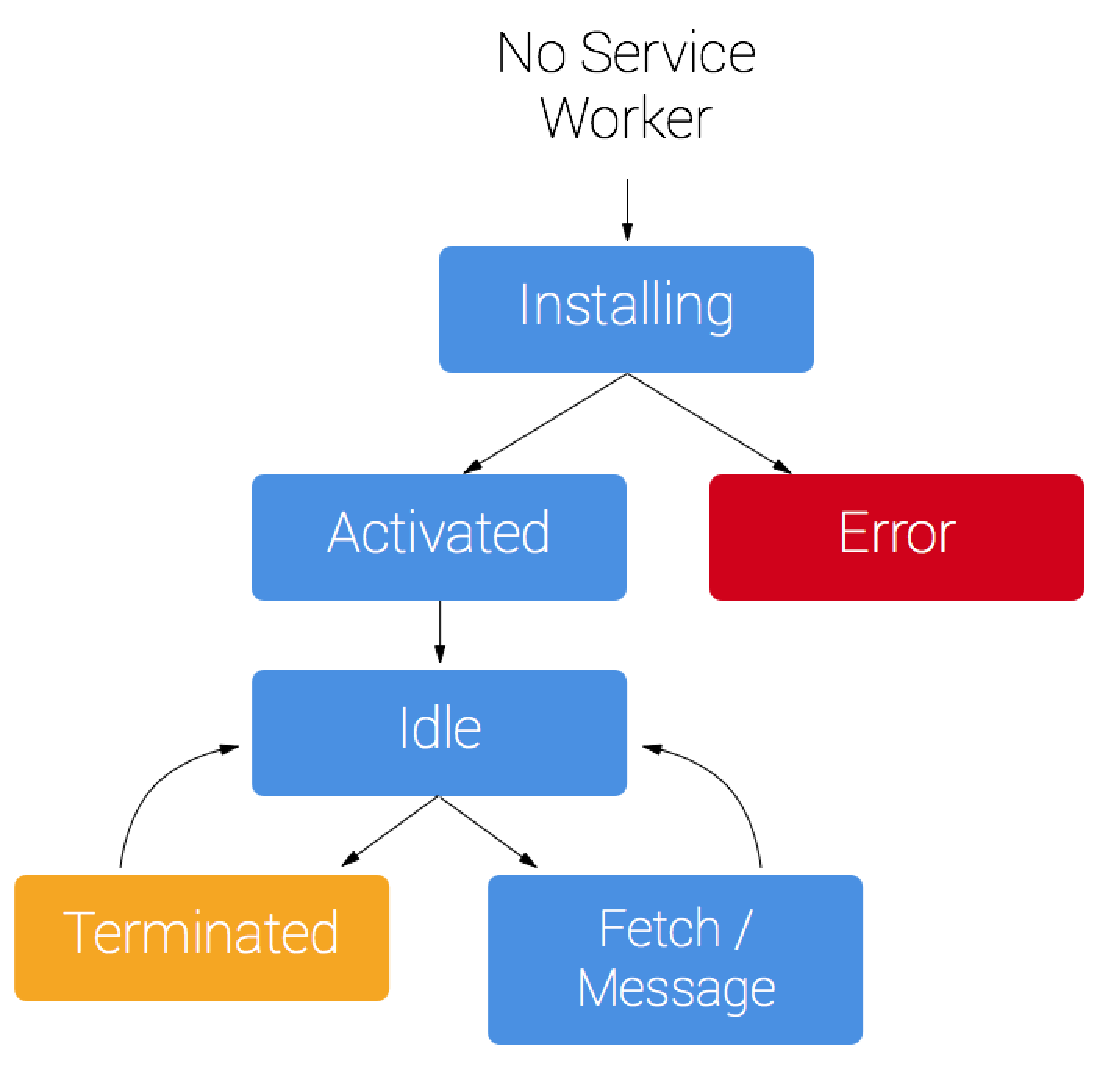
\includegraphics[width=0.8\textwidth]{figures/sw-lifecycle}
	\caption[A Figure Short-Title]{Lebenszyklus eines Service Workers\footnote{https://developers.google.com/web/fundamentals/primers/service-workers/}}
	\label{fig:swLifecycle}
\end{figure}
Nach dem ein Service Worker registriert wurde befindet er sich im Zustand der Installierung. Während der Installation werden häufig Inhalte in den Cache geladen. Wurde der Service Worker erfolgreich installiert wird er aktiviert. Ab diesem Punkt kann er Requests über das fetch event abfangen. Um Arbeitsspeicher zu sparen wird der Service Worker terminiert falls er keine fetch oder message events empfängt. Dies hat zu folge das ein Service Worker sich nicht auf den globalen Zustand verlassen kann, sondern benögten Zustand statt dessen auf die IndexedDb ausgelagert werden muss.  



%register
%activate
%
%clients.claim

%https://developers.google.com/web/fundamentals/primers/service-workers/ (bild)
%https://developer.mozilla.org/de/docs/Web/API/Service_Worker_API/Using_Service_Workers

\section{Websockets}


Websockets ist ein, auf TCP basierendes, Protokoll das bidirektionale Verbindungen zwischen Server und Webanwendung ermöglicht. Nachdem der Client eine Websocket Verbindung zum Server Aufgebaut hat ist es dem Server im Gegensatz zu HTTP möglich ohne vorherige Anfrage des Clients Daten an ihn zu senden. Zum initieren einer Verbindung wird ein Handshake durchgeführt der vom Client angestoßen werden muss. Dazu wird wie bei HTTP der Port 80 verwendet. Der Server antwortet bei erfolgreichem Handshake mit dem HTTP status code 101. Um eine Abwärtskompatibilität zu gewährleisten werden ähnliche Header wie bei HTTP verwendet.

Neben dem unverschlüsseltem URI-Schema ws definiert RFC6455\cite{rfcWebsockets} auch das verschlüsselte Schema wss. Da  sehr wenig daten overhead bei der Kommunikation besteht eigenen sich Websockets insbesondere für Anwendungen die eine geringe Latenz benötigen. Websockets werden von allen modernen Browsern unterstützt.

%bidirektionale verbindung zwischen server und Webanwendung
%auf tcp basierendes protokoll
%very little data overhead needs to be exchanged to send messages. This means a low latency communication.
%WebSockets are great for real-time and long-lived communications.
%
%
%client öffnet verbindung danach kann der server ohne vorherige aktion des cients daten senden
%
% zwei neue URI-Schemata, ws: für unverschlüsselte, und wss: für verschlüsselte Verbindungen.
% 
%handshake zur initierung der verbindung
%  wie http über port 80
%  ähnlicher header --> abwärtskompatibel
%  server antwortet mit http status 101
%  
%WebSockets are supported by all modern browsers.


RFC6455\cite{rfcWebsockets}


\section{Distributed caches}

